\documentclass{beamer}
\usepackage[T1]{fontenc} 
\usepackage[ngerman]{babel} %Umlaute,Silbentrennung
% \usepackage{beamerthemesplit} // Activate for custom appearance
 \usepackage[utf8]{inputenc} %UTF8 input file
\usepackage{cleveref}
\usepackage{multimedia}
\usepackage{graphicx}
\title{DIY Projektvortrag}
\author{Christof Pfannenmüller}
\date{\today}
\begin{document}

\frame{\titlepage} % -----------Anforderungen: 10 15 min 7 8 folien
\section[Outline]{}
\frame{\tableofcontents}


\section{mein Projekt}
\subsection{ \huge{ Wordclock auf einer Platine}}
\frame
{
  \frametitle{mein  Projekt}
{\Large Was soll\textbf{te} das Projekt enthalten?\\}\par 
\begin{itemize}
\item Wordclock
\item Möglichkeit mich aufzuwecken
\item klein genug für den Nachttisch -> max. 20cm
\item Stromreserve über die Nacht
\item viele viele verschiedene Sprachen
\end{itemize}
}



\frame
{
  \frametitle{mein  Workflow} 
  \begin{itemize}
\item Pflichten und Lastenheft
\item Layout in Eagle
\item CAD Modell
\item Frontplatte
\end{itemize}
} 
 


\frame
{
  \frametitle{Layout in Eagle}
   \begin{itemize}
\item möglichst universell
\item Größe des Vorbildes einhalten
\end{itemize}
} 

\frame
{
  \frametitle{Layout}
\begin{figure}[tb]
\centering 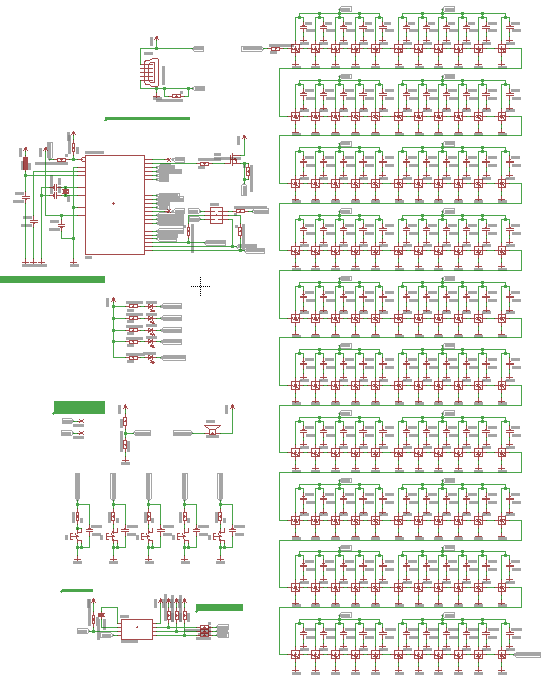
\includegraphics[width=0.65\textwidth]{EagleS1} 
\end{figure}
} 

\frame
{
  \frametitle{Layout}

\begin{figure}
     \centering
     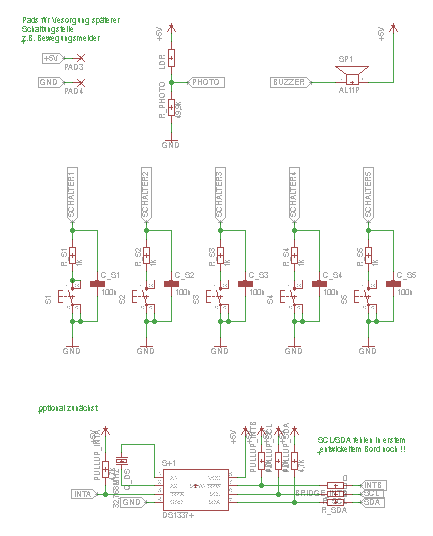
\includegraphics[width=.52\textwidth]{EagleS3}
     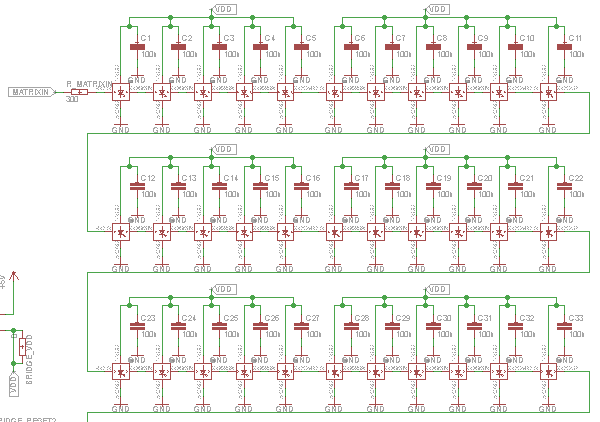
\includegraphics[width=.52\textwidth]{EagleS4}
\end{figure}

} 
 
\frame
{
  \frametitle{Qlocktwo als Größenvorbild}
\begin{figure}[tb]
\centering 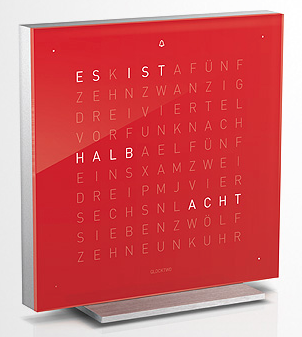
\includegraphics[width=0.65\textwidth]{Qlocktwo} 
\end{figure}
} 

 \frame{
  \frametitle{CAD Modell}
  \begin{figure}[tb]
\centering 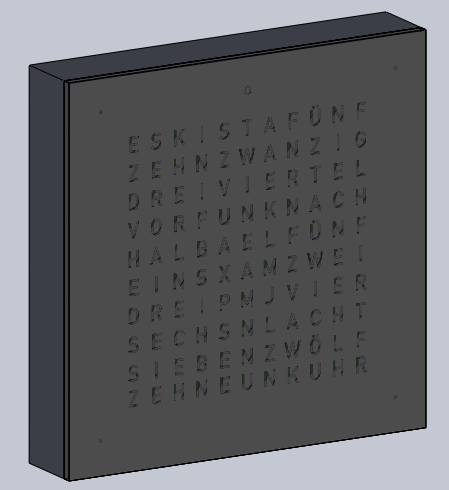
\includegraphics[width=\textwidth]{SW1} 
\end{figure}
}

 \frame{
  \frametitle{CAD Modell}
  \begin{figure}[tb]
\centering 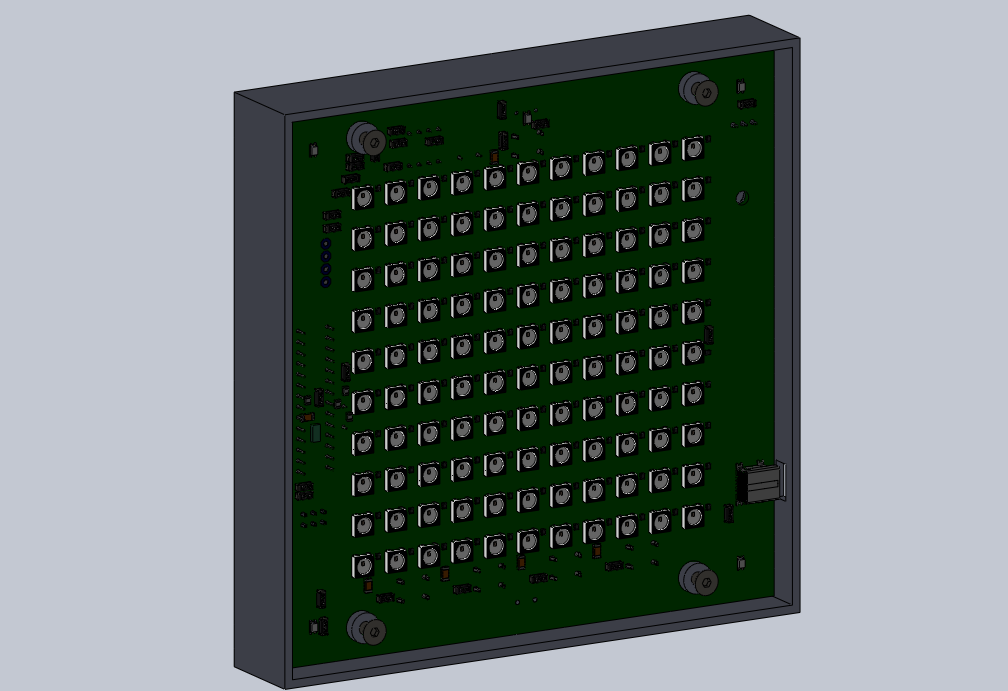
\includegraphics[width=\textwidth]{SW2} 
\end{figure}
}

 \frame{
  \frametitle{CAD Modell}
  \begin{figure}[tb]
\centering 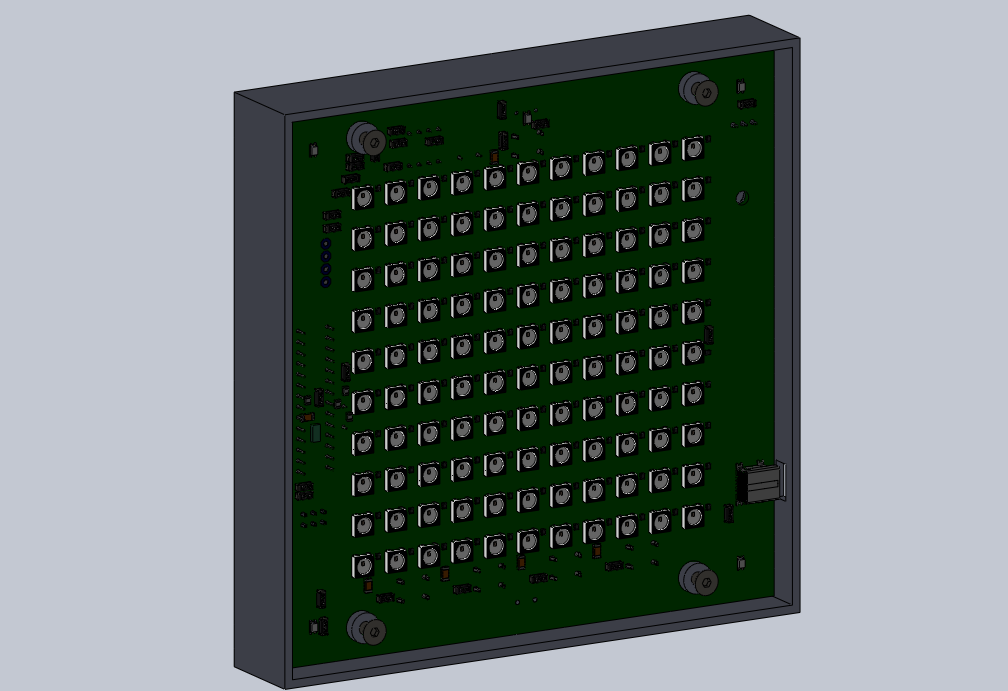
\includegraphics[width=\textwidth]{SW4} 
\end{figure}
}

 \frame{
  \frametitle{CAD Modell}
  \begin{figure}[tb]
\centering 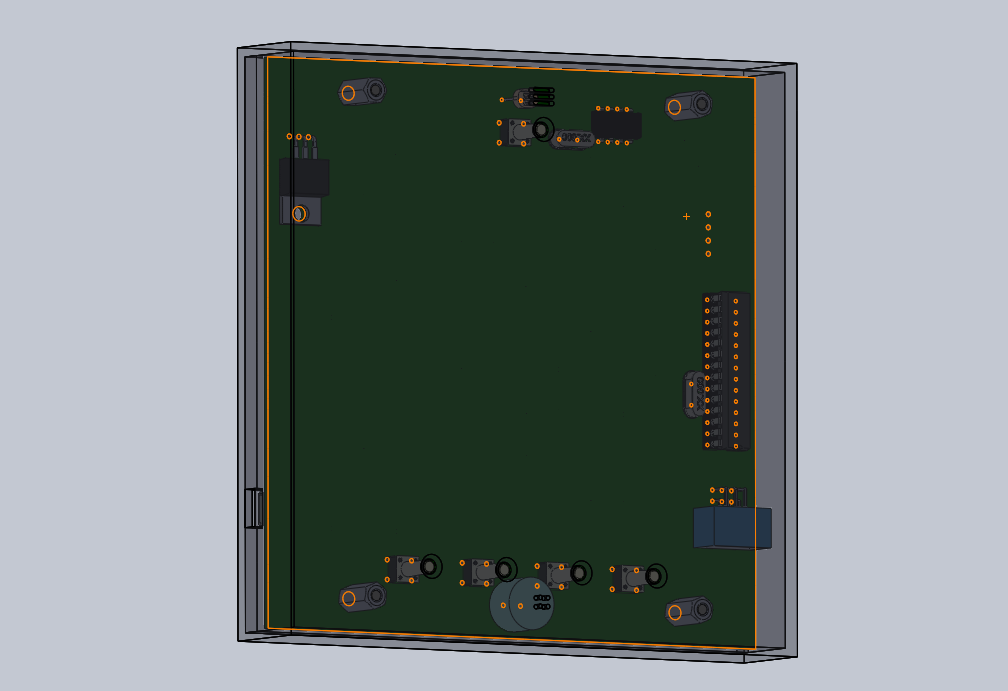
\includegraphics[width=\textwidth]{SW5} 
\end{figure}
}
\frame{
  \frametitle{CAD Modell}
  \begin{figure}[tb]
\centering 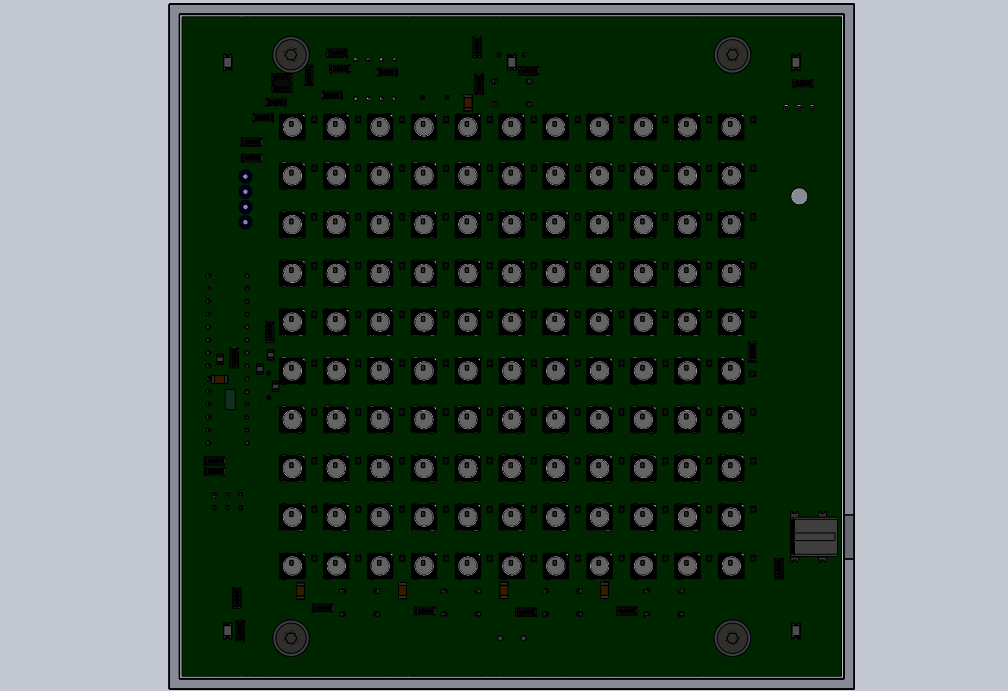
\includegraphics[width=\textwidth]{SW6} 
\end{figure}
}
\frame{
  \frametitle{CAD Modell}
  \begin{figure}[tb]
\centering 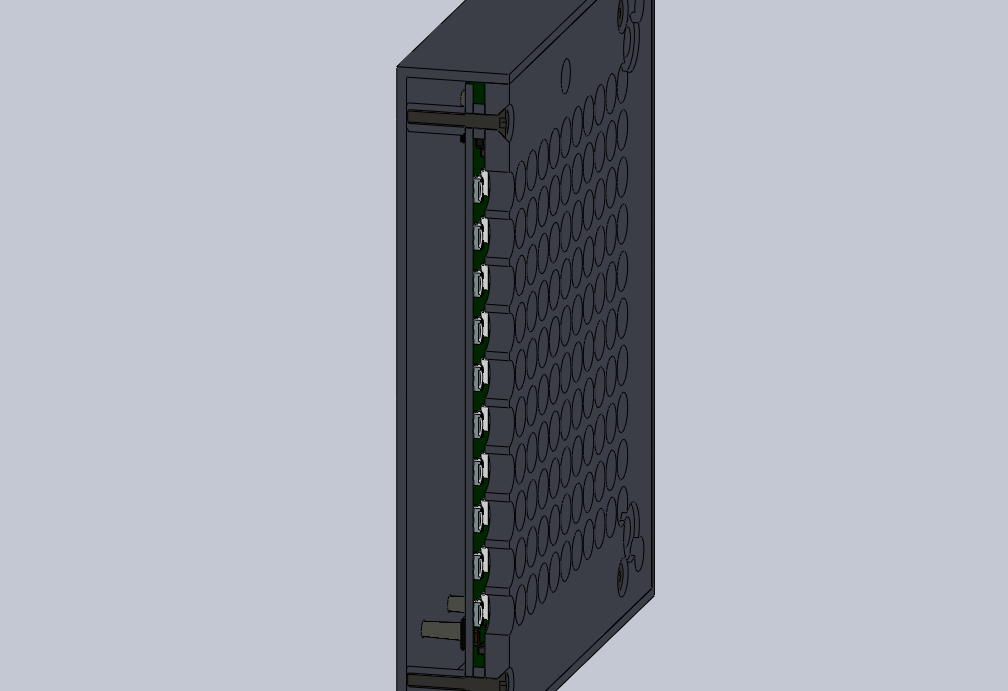
\includegraphics[width=\textwidth]{SW7} 
\end{figure}
}
 
 \frame
{
  \frametitle{Frontplatte}
  Anordnung der Buchstaben
  \begin{figure}
     \centering
     
\includegraphics[width=.52\textwidth]{Anordnung1}
     
\includegraphics[width=.52\textwidth]{Anordnung2}
\end{figure}
} 
 
\frame
{
  \frametitle{Frontplatte}
  meine Frontplatten:
  \begin{figure}
     \centering
     
\includegraphics[width=.52\textwidth]{Frontplatte1}
     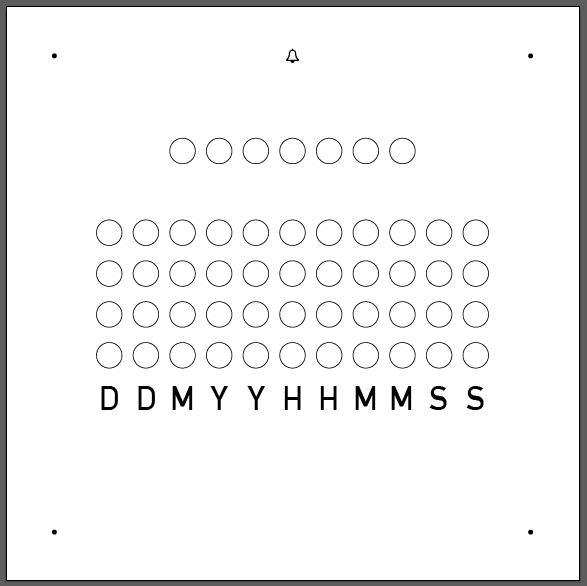
\includegraphics[width=.52\textwidth]{Frontplatte2}
\end{figure}
} 
 
 \frame
{
  \frametitle{Software}
  
} 
 
 
 
 
 
 
 
 
 \frame {\huge noch Fragen?}
\end{document}
